\section{Koncept i tre dimensioner}

\paragraph{Tvärkontraktion}
När man gör ett dragningsprov på en stång, genomgår den deformation i längdriktning samtidigt som tjockleken minskar. Detta kallas tvärkontraktion. Töjningen $\varepsilon_{t}$ av tjockleken är relaterad till töjningen i längdriktning genom
\begin{align*}
	\varepsilon_{t} = -\nu\varepsilon,
\end{align*}
där $\nu$ är Poissons konstant. Termodynamiken ger att $-1\leq\nu\leq 0.5$.

\paragraph{Skjuvspänning}
Betrakta två plattor som ligger på varandra och dras åt motsatta håll av en kraft $F$ på varje. Om de inte dras isär, balanseras dragkrafterna av krafter i kontaktytan. Låt $A$ vara kontaktytan mellan plattorna. Då definieras skjuvspänningen som
\begin{align*}
	\tau = \frac{F}{A}.
\end{align*}

\paragraph{Deformation från skjuvkrafter}
Betrakta ett rätblock med basarea $A$ och höjd $H$ som dras av motsatt riktade krafter med belopp $F$ på varje sida, illustrerad i figur \ref{fig:rectangle_twist}.
\begin{figure}[!ht]
	\centering
	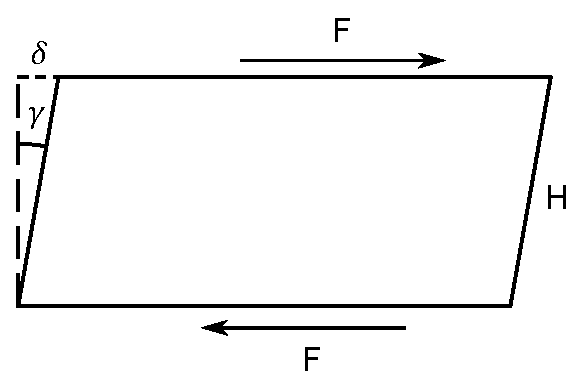
\includegraphics[width = 0.5\textwidth]{./Images/rectangle_twist.eps}
	\label{fig:rectangle_twist}
\end{figure}

Vi kan här definiera skjuvspänningen som
\begin{align*}
	\tau = \frac{F}{A},
\end{align*}
då vi kan tänka oss att plattorna som dras isär är tunna skikt i materialet. Skjuvkrafterna kommer skapa en deformation $\delta$ på en sida motsvarande vridning med en vinkel $\gamma$. Denna vinkeln uppfyller
\begin{align*}
	\tan{\gamma} = \frac{\delta}{H}.
\end{align*}
För små deformationer kan vi approximera
\begin{align*}
	\gamma = \frac{\delta}{H}.
\end{align*}
Experimentellt har man sett att
\begin{align*}
	\tau = G\gamma,
\end{align*}
där $G$ är skjuvmodulen.

\paragraph{Samband mellan materialstorheter}
För ett isotropt material gäller att
\begin{align*}
	G = \frac{E}{2(1 + \nu)}.
\end{align*}

\paragraph{Statiskt bestämta och obestämta problem}
Ett problemt är statiskt bestämt om alla inre krafter och reaktionskrafter kan bestämmas enbart med jämvikt. Detta är möjligt om det verkar maximalt $3$ krafter i planet eller $6$ i rymden.

Om ett problem ej är statiskt bestämt, är det statiskt obestämt. Då räcker icke jämviktsekvationerna, och det motsvarar att man kan ta bort ett element och vara kvar i jämvikt.

\paragraph{Elastisk vridning}
Antag att man har en stång med cirkulärt tvärsnitt fäst i ena ändan som man vrider med ett moment $M_{\text{v}}$ (i varje ända). Detta ger en vinkeldeformation $\theta$ i det yttersta tvärsnittet och $\gamma$ relativt linjen parallellt med stångens riktning. Om stången har en längd $l$ och en radius $a$, ger detta
\begin{align*}
	L\gamma = a\theta.
\end{align*}
Kombinerad med resultatet från delen om skjuvspänning ger detta
\begin{align*}
	\frac{\theta}{L} = \frac{\tau}{G}.
\end{align*}
Antag nu att $\tau = \frac{M_{\text{v}}}{K}$. Detta ger
\begin{align*}
	\frac{\theta}{L} = \frac{M_{\text{v}}}{GK}.
\end{align*}
$K$ är en konstant som beror av stångens geometri.

Hur beräknar vi $K$? Jo, man integrerar momentets differential över tvärsnittet. Vi vet att detta differentialet ges av kraft gånger arm, och det är så skjuvspänningen kommer in.

\paragraph{Balkböjning - fundamentala koncept}
För att beskriva balkar behöver vi införa fler olika sorters inre krafter och moment. Dessa illustreras i figur \ref{fig:beam_forces}.
\begin{figure}[!ht]
	\centering
	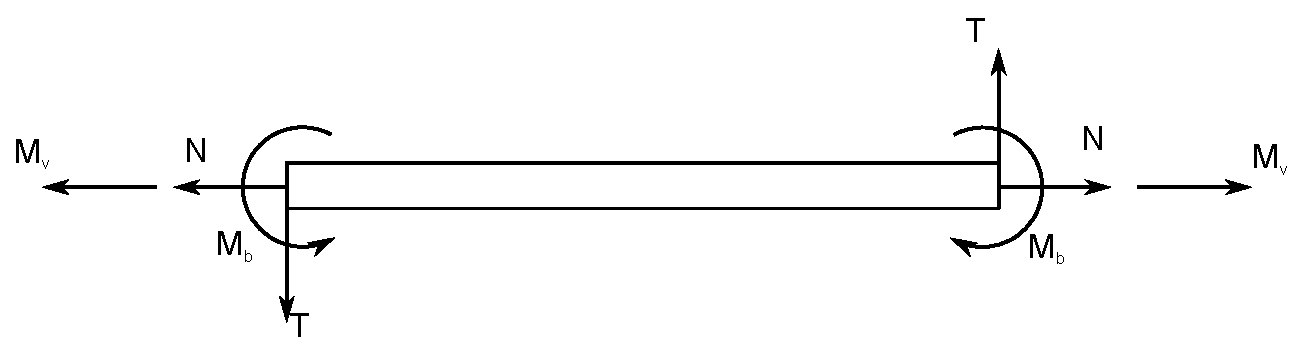
\includegraphics[width = 0.5\textwidth]{./Images/beam_forces.eps}
	\caption{Illustration av inre krafter och moment i en balk.}
	\label{fig:beam_forces}
\end{figure}
Vi har infört normalkraften $N$, tvärkraften $T$, det böjande momentet $M_{\text{b}}$ och det vridande momentet $M_{\text{v}}$.

Låt $u$ vara balkens deformation normalt på dens utsträkning. Vi har från enaxliga tillståndet att
\begin{align*}
	\frac{\Delta u}{L} = \frac{N}{EA}.
\end{align*}
Låt $\theta$ och $\phi$ vara vinklarna för böjning och vridning. Vi har från innan att
\begin{align*}
	\frac{\Delta\theta}{L} = \frac{M_{\text{v}}}{GK},
	\frac{\Delta\phi}{L} = \frac{M_{\text{b}}}{EI}.
\end{align*}

\paragraph{Allmänt tillstånd för en balk}
Snitta nu ut ett element med längd $\dd{x}$ från en balk. Om balken påverkas av en last $q$ per längdenhet, ger kraftjämvikten
\begin{align*}
	T(x + \dd{x}) - T(x) + q(x)\dd{x} = 0,
\end{align*}
vilket ger
\begin{align*}
	\dd{T}{x} = -q.
\end{align*}
Momentjämvikt kring centrum ger
\begin{align*}
	M(x + \dd{x}) - M(x) - (T(x) + T(x + \dd{x}))\dd{x} = 0.
\end{align*}
Bidraget från tvärkraften ges av
\begin{align*}
	T(x) + T(x + \dd{x}) &= 2T(x) + \dv{T}{x}\dd{x} \\
	                     &= 2T(x) - q(x)\dd{x}.
\end{align*}
Insatt i momentjämvikten fås
\begin{align*}
	M(x + \dd{x}) - M(x) - \frac{1}{2}\dd{x}(T(x) + T(x + \dd{x})) = M(x + \dd{x}) - M(x) - T(x)\dd{x} + \frac{1}{2}\dd{x}q(x)\dd{x}.
\end{align*}
Vi försummar nu alla andra ordningens termer, vilket ger
\begin{align*}
	\dv{M}{x} = T.
\end{align*}
Kombinerat med det förra resultatet fås
\begin{align*}
	\dv[2]{M}{x} = -q.
\end{align*}

\paragraph{Randvillkor för balkar}
En balk kan i en given ända vara
\begin{itemize}
	\item fri, vilket ger $T = 0$ och $M = 0$.
	\item fritt upplagd, vilket ger $M = 0$.
	\item glidinspänd, vilket ger $T = 0$.
	\item fast inspönd, vilket ej ger villkor för de inre krafterna och momenterna.
\end{itemize}

\paragraph{Balkböjning vid normalspänning}
Vid böjning inför vi en $z$-koordinat normal på medellinjen genom balken, och centrerar våra koordinater i tvärsnittets tyngdpunkt. Vi antar till att börja med att tvärsnittet är symmetrisk med avseende på $z$-axeln, samt att
\begin{itemize}
	\item plana tvärsnitt förblir plana.
	\item tvärsnitt förblir vinkelräta mot medellinjen.
	\item det för varje $z$ är ett enaxligt samband mellan $\sigma$ och $\varepsilon$.
	\item alla deformationer är små och för balkar vars längd är mycket större än deras tjocklek.
\end{itemize}
De två första uppfylls om skjuvspänningen är försumbar jämförd med normalspänningen.

Betrakta nu ett litet element med ursprunglig längd $L_{0}$ vars medellinje har böjts så den har krökningsradie $R$. Geometri ger oss
\begin{align*}
	(R + z)\phi = L_{0}(1 + \varepsilon(z)).
\end{align*}
I $z = 0$ har vi
\begin{align*}
	R\phi = L_{0}(1 + \varepsilon_{0}),
\end{align*}
vilket ger
\begin{align*}
	L_{0}(1 + \varepsilon_{0}) + z\phi &= L_{0}(1 + \varepsilon(z)), \\
	\varepsilon(z)                     &= \varepsilon_{0} + \frac{\phi}{L_{0}}z.
\end{align*}
Vi kan även substituera för $\phi$ för att få
\begin{align*}
	\varepsilon(z) = \varepsilon_{0} + \frac{1 + \varepsilon_{0}}{R}z.
\end{align*}

Om vi snittar och får någon given normalkraft $N$ på ytan, gäller det att
\begin{align*}
	N &= \integ{A}{}{F}{} \\
	  &= \integ{A}{}{A}{\sigma}.
\end{align*}
Hookes lag ger
\begin{align*}
	N &= \integ{A}{}{A}{E\left(\varepsilon_{0} + \frac{z}{R}\right)} \\
	  &= \integ{A}{}{A}{E\varepsilon_{0} + E\frac{z}{R}}.
\end{align*}
Om vi antar att elasticitetsmodulen är konstant över ytan, kan vi dra ut konstanter. Den andra integralen är då tyngdpunktens $z$-koordinat (om vi antar homogen massfördelning), som per definition var $0$. Detta ger
\begin{align*}
	N = E\varepsilon_{0}A.
\end{align*}

Vi beräknar vidare momentet $M_{y}$ normalt på både längdriktningen och $z$-koordinaten. Detta ges av
\begin{align*}
	M_{y} &= \integ{A}{}{A}{\sigma z} \\
	      &= \integ{A}{}{A}{Ez\left(\varepsilon_{0} + \frac{z}{R}\right)} \\
	      &= \integ{A}{}{A}{Ez\varepsilon_{0} + \frac{E}{R}z^{2}}.
\end{align*}
Första integralen är igen lika med $0$. Andra är relaterad till yttröghetsmomentet
\begin{align*}
	I_{y} = \integ{A}{}{A}{z^{2}}.
\end{align*}
Vi får alltså
\begin{align*}
	M = \frac{EI_{y}}{R}.
\end{align*}
Vi kan nu sätta ihop dessa resultat och få
\begin{align*}
	\sigma = \frac{N}{A} + \frac{M_{y}}{I_{y}}z.
\end{align*}

Vid ren böjning, dvs. ingen normalkraft, kan vi skriva
\begin{align*}
	\abs{\sigma}_{\text{max}} = \frac{\abs{M_{y}}\abs{z}_{\text{max}}}{I_{y}}.
\end{align*}
Vi kan införa böjmotståndet
\begin{align*}
	W_{\text{b}} = \frac{I_{y}}{\abs{z}_{\text{max}}},
\end{align*}
och får då
\begin{align*}
	\abs{\sigma}_{\text{max}} = \frac{\abs{M_{y}}}{W_{\text{b}}}.
\end{align*}